\begin{mainquestion}{impedanceforms}{Impedance Conversion Table}

\begin{partquestion}{filltable}{Fill out the following table. Assume an angular frequency of \qty{1}{\radian/\second}}
% Imported from a solutions document. The prompt table below is reconstructed with only the given Cartesian impedances populated.

{\small
\renewcommand{\arraystretch}{1.25}
\begin{center}
\resizebox{\textwidth}{!}{%
\begin{tabular}{|c|c|c|c|c|c|c|c|c|c|}
\hline
Cartesian form of $Z$ & Polar form of $Z$ & Euler form of $Z$ & Series equivalent circuit for $Z$ & Parallel equivalent circuit for $Z$ & Admittance & Resistance & Reactance & Conductance & Susceptance \\
\hline
$1 + 2j\ \Omega$ & & & & & & & & & \\
\hline
$1.5 + 1.5\sqrt{3}j\ \Omega$ & & & & & & & & & \\
\hline
$2\sqrt{2} - 2\sqrt{2}j\ \Omega$ & & & & & & & & & \\
\hline
$5 - \frac{1}{6}j\ \Omega$ & & & & & & & & & \\
\hline
$3.965 + 3.469j\ \Omega$ & & & & & & & & & \\
\hline
$\frac{3}{25} - \frac{4}{25}j\ \Omega$ & & & & & & & & & \\
\hline
\end{tabular}%
}
\end{center}
}

\begin{answer}
{\small
\renewcommand{\arraystretch}{1.25}
\begin{center}
\resizebox{\textwidth}{!}{%
\begin{tabular}{|c|c|c|c|c|c|c|c|c|c|}
\hline
Cartesian form of $Z$ & Polar form of $Z$ & Euler form of $Z$ & Series equivalent circuit for $Z$ & Parallel equivalent circuit for $Z$ & Admittance & Resistance & Reactance & Conductance & Susceptance \\
\hline
$1 + 2j\ \Omega$ & $\sqrt{5}\angle 63.43^{\circ}$ & $\sqrt{5}e^{j\tan^{-1}(2)}$ & 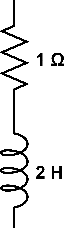
\includegraphics[height=0.95in]{questionbank/circuit_quantities/impedance_forms/v0/row1_series.png} & 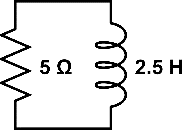
\includegraphics[height=0.6in]{questionbank/circuit_quantities/impedance_forms/v0/row1_parallel.png} & $0.2 - 0.4j\text{ S}$ & $1\ \Omega$ & $2\ \Omega$ & $0.2\text{ S}$ & $-0.4\text{ S}$ \\
\hline
$1.5 + 1.5\sqrt{3}j\ \Omega$ & $3\angle 60^{\circ}$ & $3e^{j\frac{\pi}{3}}$ & 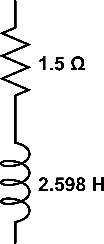
\includegraphics[height=0.95in]{questionbank/circuit_quantities/impedance_forms/v0/row2_series.png} & 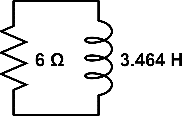
\includegraphics[height=0.6in]{questionbank/circuit_quantities/impedance_forms/v0/row2_parallel.png} & $\frac{1}{6} - \frac{\sqrt{3}}{6}j\text{ S}$ & $1.5\ \Omega$ & $1.5\sqrt{3}\ \Omega$ & $\frac{1}{6}\text{ S}$ & $-\frac{\sqrt{3}}{6}\text{ S}$ \\
\hline
$2\sqrt{2} - 2\sqrt{2}j\ \Omega$ & $4\angle -45^{\circ}$ & $4e^{-j\frac{\pi}{4}}$ & 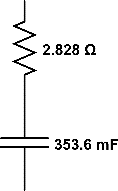
\includegraphics[height=0.95in]{questionbank/circuit_quantities/impedance_forms/v0/row3_series.png} & 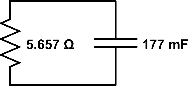
\includegraphics[height=0.6in]{questionbank/circuit_quantities/impedance_forms/v0/row3_parallel.png} & $\frac{\sqrt{2}}{8} + \frac{\sqrt{2}}{8}j\text{ S}$ & $2\sqrt{2}\ \Omega$ & $-2\sqrt{2}\ \Omega$ & $\frac{\sqrt{2}}{8}\text{ S}$ & $\frac{\sqrt{2}}{8}\text{ S}$ \\
\hline
$5 - \frac{1}{6}j\ \Omega$ & $5.003\angle -1.9^{\circ}$ & $5.003e^{j\tan^{-1}\left(-\frac{1}{30}\right)}$ & 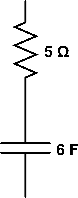
\includegraphics[height=0.95in]{questionbank/circuit_quantities/impedance_forms/v0/row4_series.png} & 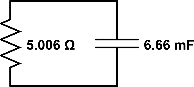
\includegraphics[height=0.6in]{questionbank/circuit_quantities/impedance_forms/v0/row4_parallel.png} & $0.200 + 0.0067j\text{ S}$ & $5\ \Omega$ & $-\frac{1}{6}\Omega$ & $0.200\text{ S}$ & $0.0067\text{ S}$ \\
\hline
$3.965 + 3.469j\ \Omega$ & $5.27\angle 41.2^{\circ}$ & $5.27e^{j(0.719)}$ & 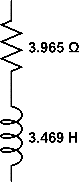
\includegraphics[height=0.95in]{questionbank/circuit_quantities/impedance_forms/v0/row5_series.png} & 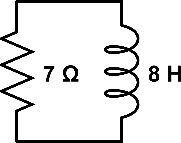
\includegraphics[height=0.6in]{questionbank/circuit_quantities/impedance_forms/v0/row5_parallel.png} & $0.143 - 0.125j\text{ S}$ & $3.965\ \Omega$ & $3.469\ \Omega$ & $0.143\text{ S}$ & $-0.125\text{ S}$ \\
\hline
$\frac{3}{25} - \frac{4}{25}j\ \Omega$ & $0.2\angle -53.1^{\circ}$ & $0.2e^{-j(0.927)}$ & 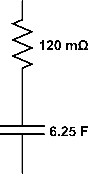
\includegraphics[height=0.95in]{questionbank/circuit_quantities/impedance_forms/v0/row6_series.png} & 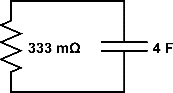
\includegraphics[height=0.6in]{questionbank/circuit_quantities/impedance_forms/v0/row6_parallel.png} & $3 + 4j\text{ S}$ & $\frac{3}{25}\ \Omega$ & $-\frac{4}{25}\ \Omega$ & $3\text{ S}$ & $4\text{ S}$ \\
\hline
\end{tabular}%
}
\end{center}
}

To convert in general, starting with a Cartesian form of $Z = a + jb$, the polar form will be $\sqrt{a^{2} + b^{2}}\angle\tan^{-1}\left(\frac{b}{a}\right)$, and Euler's form is $\sqrt{a^{2} + b^{2}}e^{j\tan^{-1}\left(\frac{b}{a}\right)}$. The serial equivalent circuit will be a resistor of value $a$ and an inductor of value $b$ if $b > 0$, or a capacitor of value $-\frac{1}{b}$ if $b < 0$. The parallel equivalent circuit will be a resistor of value $\frac{a^{2} + b^{2}}{a}$ and an inductor of value $\frac{a^{2} + b^{2}}{b}$ if $b > 0$, or a capacitor of value $-\frac{b}{a^{2} + b^{2}}$ if $b < 0$. The admittance is
\[
\frac{1}{a + jb} = \frac{a - jb}{a^{2} + b^{2}} = \frac{a}{a^{2} + b^{2}} - j\frac{b}{a^{2} + b^{2}}
\]
(compare with the parallel equivalent circuit). From here, the resistance is $a$, the reactance is $b$, the conductance is $\frac{a}{a^{2} + b^{2}}$ and the susceptance is $\frac{-b}{a^{2} + b^{2}}$.
Starting with any of the first six columns, you can work out the other entries based on the relationships described above.
\end{answer}
\end{partquestion}

\end{mainquestion}